\documentclass{beamer}

\usepackage[utf8]{inputenc}
\usecolortheme{beaver}
\usepackage{caption}
\usepackage{amsmath}
\usepackage{amsfonts}
\usepackage{amssymb}
\usepackage{subcaption}
\usepackage{mathtools}
\usepackage{bm}
\usepackage{xcolor}
\usepackage{soul}
\usepackage{tikz}
\usepackage{graphicx}
\usepackage[style=verbose, backend=biber]{biblatex}
\newcommand{\mathcolorbox}[2]{\colorbox{#1}{$\displaystyle #2$}}

\title{Partially Adaptive Regularized Multiple Regression Analysis for Estimating Linear Causal Effects}
\author{Hisayoshi Nanmo, Manabu Kuroki}
\date{}

\begin{document}
\maketitle

\begin{frame}
	\frametitle{Regularization in Linear Regression}
	\begin{itemize}
		\item Linear Regression Model: $ \bm{Y} = \bm{XB} + \bm{e} $
		\item OLS: $ \bm{\hat{B}} = min_{\bm{B}} (\bm{Y} - \bm{XB})^2 $
		\item OLS fails when have high-dimensional covariates or multicolinearity in covariates. Regularization can be used:
			\begin{itemize}
				\item Ridge Regression (L2): $ \bm{\hat{B}} = min_{\bm{B}} [(\bm{Y}-\bm{XB})^2 + \mathcolorbox{yellow}{\lambda \sum \bm{B}^2}] $
				\item Lasso Regression (L1): $ \bm{\hat{B}} = min_{\bm{B}} [(\bm{Y}-\bm{XB})^2 + \mathcolorbox{yellow}{\lambda \sum \mid \bm{B} \mid}] $
				\item Elastic net: $ \bm{\hat{B}} = min_{\bm{B}} [(\bm{Y} - \bm{XB})^2 + \mathcolorbox{yellow}{\lambda_2 \sum \bm{B}^2 + \lambda_1 \sum \mid \bm{B} \mid}] $
			\end{itemize}
	\end{itemize}
\end{frame}

\begin{frame}
	\frametitle{Linear Regression in Causal Inferene}
	\begin{figure}
		\centering
		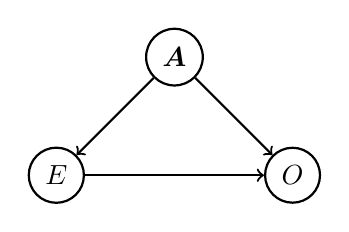
\begin{tikzpicture}
			\begin{scope}[every node/.style={circle, thick, draw}]
				\node (E) at (0, 0) {$ E $};
				\node (O) at (3, 0) {$ O $};
				\node (A) at (1.5, 1.5) {$ \bm{A} $};
			\end{scope}

			\path [draw, thick, ->] (E) -- (O);
			\path [draw, thick, ->] (A) -- (E);
			\path [draw, thick, ->] (A) -- (O);
		\end{tikzpicture}
		\begin{itemize}
			\item Estimate the effect of exposure $ E $ on outcome $ O $.
			\item First step would be to find an adjustment set. In this case, $ \bm{A} $.
			\item Under linearity assumption, the effect can be estimated by doing a 
				linear regression: $ O \sim E + A $.
			\item The regression coefficient of $ E $ is the effect.
			\item In the case of high dimensional or multicolinear
				adjustment sets, OLS can be used.
			\item Using any regularization method in this case
				would also affect the causal effect estimate
				and leads to bias.
		\end{itemize}
	\end{figure}
\end{frame}

\begin{frame}
	\frametitle{Contribution Summary}
	\begin{itemize}
		\item New L1 regularization approach that:
			\begin{enumerate}
				\item Provides consistent estimates even with
					multicollinearity/high-dimensional data
					problems.
				\item Doesn't remove the important variables
					from the regression model.
			\end{enumerate}
		\item New optimization algorithm as normal L1 optimization algorithms are not applicable because of the some unregularized terms.
		\item Theoretical Results: Extend collapsibility to regularized regression analysis.
	\end{itemize}
\end{frame}

\begin{frame}
	\frametitle{PALpMA: Partial Regularization}
	$ \bm{Y} \sim \bm{B_x X} + \bm{B_z Z} + \bm{B_w W} $ where $ \bm{W} \cup \bm{Z} = \bm{A} $ and $ \bm{W} \cap \bm{Z} = \phi $.
	
	Loss function: $ min_{B_x, B_z, B_w} (Y - B_x X - B_z Z - B_w W)^2 + \lambda_p \mid \gamma \odot B_w \mid $

\end{frame}

\begin{frame}
	\frametitle{Optimization Algorithm: i-PROGLES}
\end{frame}

\begin{frame}
	\frametitle{Collapsibility}
\end{frame}

\begin{frame}
	\frametitle{Numerical Results}
\end{frame}

\begin{frame}
	\frametitle{Discussion Points}
	\begin{itemize}
		\item Best strategies for selecting the confounding set, $
			\bm{W} $, and the set of possible confounders, $ \bm{Z} $.
		\item Choosing the optimal hyperparameters. Grid search for best 
			predictive performance or any other better strategies?
		\item Extending it to other statistical models like Generalized
			Linear Models, Generalized Estimating Equations, etc.
	\end{itemize}
\end{frame}

\end{document}
